\ifx\allfiles\undefined
\documentclass{XDBAthesis}
\def\pictures{}
\begin{document}
\else
\fi
\chapter{基于节点相似度的图相似性搜索}
\label{chap:gHash}
由前文可知,图数据能表示复杂的数据结构,在诸多领域也得到了广泛应用。从基本的生物,化学的分子结构,到交通网络,人际关系网都可以用图来建模。而对于图数据库的索引也自然成为了热点问题。

上一章我们介绍了精确子图搜索方法,但是由于真实情况下图数据库具有信息不完整,含有杂质等情形,精确搜索容易出现各种不匹配问题,难以得到我们想要的结果。同时,对于查询图的完整信息有时查询者也并不了解。所以相似性搜索的实际应用领域更加广泛。对于实际应用,相似性搜索的研究意义远超过了精确搜索。

传统的图相似性算法虽然运行效率已较为理想,但是编码上过于复杂,也无法做到对所有图数据库良好适配。所以本章我们提出了一种性能上不输于传统算法,但是实现更为简单,并且无需复杂设计即可适用于大量图数据库的基于节点相似度的通用型算法。本章将首先详细介绍下一些相关概念,然后介绍下我们算法的具体思路并给出详细的代码设计方案,最后给出对于真实数据的实验结果与分析。
\section{相关概念}
本节主要介绍下下文介绍算法时会用到的一些概念,包括小波图匹配核函数,G-Hash中的图相似度定义,节点相似度定义三部分。
\subsection{小波图匹配核函数}
\emph{小波图匹配核函数(Wavelet Graph matching kernel)}\cite{ghash}是Wang等人在G-Hash算法中提出的,用于度量图相似度的一个核心函数。其思想是先通过压缩每个节点周围邻接节点的属性信息,然后应用非递归线性核去计算图之间的相似度。这个方法包含两个重要的概念:\emph{h-hop邻域}和\emph{离散小波变换}。用$N_h (v)$标记一个节点$v$的\emph{h跳邻域},代表一个距离节点$v$最短距离是$h$跳(跳过$h$个节点,也就是$h+1$的曼哈顿距离)的节点集合。\emph{离散小波变换}涉及到一个小波函数的定义,见下文公式\eqref{eq:wavelet} ,也用到了$h$跳邻域。
\begin{equation}
    \psi_{j,k}=\frac{1}{h+1}\int_{j/(k+1)}^{(j+1)/(k+1)}\varphi(x)dx
    \label{eq:wavelet}
\end{equation}
$\varphi(x)$代表\emph{Haar}或者\emph{Mexican Hat}小波函数,$h$是在将$\varphi(x)$在$[0,1)$区间上分成$h+1$个间隔后的第$h$个间隔,$j\in[0,h]$。
基于以上两个定义,我们现在可以将小波分析用在图上了。我们用小波函数来计算每个节点的局部拓扑和。公式\eqref{eq:wm}展示了一个小波度量方法,记做$\Gamma_h (v)$,以图$G$中的一个节点$v$为例。
\begin{equation}
    \Gamma_h (v)=C_{h,v}\times\sum_{j=0}^k \psi_{j,k}\times\bar{f}_j (v)
    \label{eq:wm}
\end{equation}
其中,$C_{h,v}$是一个归一化因子
\begin{equation}
    C_{h,v}=(\sum_{j=0}^h \frac{\psi_{j,h}^2 }{|N_h (v)|})^{-1/2},
\end{equation}
$\bar{f}_{j}(v)$是离节点$v$最远距离为$j$的原子特征向量的平均值
\begin{equation}
    \bar{f}_{j}(v)=\frac{1}{|N_{j}(v)|}\sum_{u\in N_{j}(v)}f_u
\end{equation}
$f_u $表示节点$v$的特征向量值。这样的特征向量值只会是下面四种中的一种:定类,定序,定距,定比。对于定比和定距特征值,直接在上述的小波分析时代入其值即可得到局部特征值。对于定类和定序节点特征,我们首先建立一个直方图,然后用小波分析提取出特征值。在节点$v$分析完成后,我们可以得到一个节点列表$\Gamma^h (v)=\{\Gamma_{1}(v),\Gamma_{2}(v),...,\Gamma_{h}(v)\}$,我们称其为小波测度矩阵。用此方法我们可以将一个图转换为一个节点向量集合。因为小波变换有明确的正负区域,所以这些小波压缩特征可以表示出局部的邻接节点和距离较远的邻接节点的差异。因此,通过小波变换,一幅图的结构化信息可以压缩成节点特征。从而我们可以忽略拓扑结构来专心于节点匹配。核函数就是建立在这些集合上的,我们以图$G$和$G'$为例,图匹配核函数是这样的
\begin{gather}
    k_{m}(G,G')=\sum_{(u,v)\in V(G)\times V(G')}K(\Gamma^{h}(u),\Gamma^h (v) ), \\
    K(X,Y)=e^{\frac{-\|X-Y\|_{2}^{2}}{2}}.
\end{gather}
WA方法是一种很好的利用核函数进行图相似度定义的方法。但是这个方法有一个问题,就是小波匹配核的总时间复杂度是$O(m^2 )$,核矩阵的是$O(n^2 \times m^2 )$,$n$是数据库图个数,$m$是平均节点个数。这意味着,当数据库尺寸增加时,计算时间将大幅度增加。

\subsection{G-Hash中的图相似性定义}
图相似性有很多种定义方式有很多,第\ref{chap:background}章中介绍的\emph{图编辑距离}和\emph{最大公共子图}就是两种常用的图相似度度量方法。

G-Hash中是利用核函数计算两图相似性的。公式\eqref{eq:ghashDistance}就是两图相似度距离的定义。
\begin{equation}
\begin{split}
    &d(G,G')=\sqrt{\|\phi(G)-\phi(G')\|_{2}^{2}}\\
              &=\sqrt{\langle\phi(G)-\phi(G'),\phi(G)-\phi(G')\rangle}\\
              &=\sqrt{\langle\phi(G),\phi(G)\rangle+\langle\phi(G'),\phi(G')\rangle-2\langle\phi(G),\phi(G')\rangle}\\
              &=\sqrt{k_{m}(G,G)+k_{m}(G',G')-2k_{m}(G,G')}
\end{split}
\label{eq:ghashDistance}
\end{equation}

公式中$k_{m}(G,G)$代表图$G$和其本身的核函数值,$k_{m}(G',G')$是图$G'$及其本身的值,$k_{m}(G,G')$就是图$G$和$G'$的。

\begin{equation}
k_{m}(G,G')=\sum_{v\in G',u\in simi(v)}K(\Gamma^{h}(u),\Gamma^{h}(v))
\end{equation}

$simi(v)$是一个包含着图$G$和节点$v$哈希到同一个位置的节点集合。我们用以下的解码方式来获取包含这些节点的图号和节点号。

显然,仅利用相似点对而非所有点对来计算两图相似度可以节约很多运算时间。因此为了增加准确度,相似的节点应该被哈希到相邻的位置。在图很大(如大于40)时,我们也要计算相邻位置的节点。

因此在核函数计算时我们只考虑相似点对,在使用RBF核的情况下,$K(\Gamma^{h}(u),\Gamma^{h}(v))\approx1$,所以公式(2)可以写成
\begin{equation}
    K(G,G')\approx\sum_{v\in G',u\in simi(v)}1=\sum_{v\in G'}|simi(v)| 
\end{equation}

$|simi(v)|$是在$simi(v)$中的节点数目。这意味着我们只需要数据图$G$中和查询$G'$相似的点个数,其和就是我们要求的核。同理,我们可以这样计算每个图与其自己的核。显然,每个图与自己的核就是节点数目。

所以公式\eqref{eq:ghashDistance}最终变成公式\eqref{eq:ghashfinal},其中$|V_{G}|$代表图$G$的节点数。
\begin{equation}
    d(G,G')=\sqrt{|V_{G}|+|V_{G'}| -2\sum_{v\in G'}|simi(v)| }
    \label{eq:ghashfinal}
\end{equation}

%在完成上述操作后,我们会得到一个相似度列表,其每一个值都对应这一个数据库中的图与查询图的相似度,通过对这个列表排序,我们就可以得到对于给定的查询的$K-NNs$。
\subsection{节点相似度}
在上一节我们介绍了G-Hash中的图相似性的定义。其中有参数$simi(v)$代表与节点$v$相似的节点,但是何为相似,这个很难定义。G-Hash算法在这边根据不同图数据库构建了不同类型的哈希,来保证相似的节点都在相邻位置。而这在实际应用中很是困难。因此我们提出了\emph{节点相似度}这一概念。我们用查询图每个节点和数据图中每个节点的节点相似度作为$simi(v)$的值。
\begin{defn}[节点相似度]
    用\emph{简化包(Reduced Bag)}表示的两个节点字符串之间的相似度节点相似度称为\emph{节点相似度}。
\end{defn}
因为简化包表示的字符串实质上是一个向量,如$'a,1,0,1'$就可以看做一个向量$\vec{A}=(a,1,0,1) $,所以对于字符串的距离,也就是节点相似度,可以用公式\eqref{eq:stringdis}计算。
\begin{equation}
    simi(A,B)=\frac{\vec{A}\times \vec{B}}{||\vec{A}|\times |\vec{B}||} \leq 1
    \label{eq:stringdis}
\end{equation}
其中,$|\vec{A}|$表示$\vec{A}$的模,$simi(A,B)$永远是小于等于1的,值越大代表越为相似,为1代表两个节点特征完全一样。
\section{基于节点相似度的图相似性搜索}
本算法和G-Hash\cite{ghash}基本类似,只是在查询过程计算相似度时没有利用哈希特征找到相似的节点,而是利用节点相似度来计算相似度。这样避免了由于哈希函数选取不当造成的相似节点不在靠近位置的问题。用普通的枚举虽然理论复杂度从$O(1)$变为了$O(n)$但是提高了查询准确度,并且由于哈希存在冲突,而实际图节点一般最多为千个等情况,我们算法的运行效率并不比G-Hash低,甚至在某些情况下会略好于G-Hash算法,而且编码难度也大大降低。本节将从数据库构建,查询过程,数据库维护,编码设计四个方面详细说明我们提出的基于节点相似度的图相似性搜索算法。
\subsection{数据库构建}
首先统计数据库中的不同标号数目,然后将数据库中的每幅图都用简化包表示,选取节点标号和与其直接连接的各标号个数作为特征值。归一化后变成字符串,利用红黑树建立Bag编号与字符串的对应关系。之所以选用红黑树而不是哈希表是因为对于纯字符串结构红黑树的表现要好于哈希表。然后再以Bag编号为图,图序号为列建立一个二维表,每个值代表在此图中此种节点有几个。最终数据库如表\ref{tb:ghashdatabase}所示。
%
%\begin{figure}
%    
%    \caption{红黑树示例}
%    \label{fg:ghashdatabase}
%\end{figure}
\begin{table}[htb]
    \centering
    \begin{tabular}{|c|c|c|c|}
    \hline
        Bag编号 & $G_1 $ & $G_2 $ & $G_3 $ \\\hline
        1 & 0 & 3 & 1 \\\hline
        2 & 1 & 0 & 2 \\\hline
        3 & 4 & 2 & 1 \\\hline
        4 & 2 & 3 & 0 \\\hline
    \end{tabular}
    \caption{数据库示例}
    \label{tb:ghashdatabase}
\end{table}
\subsection{查询前K个相似图}
首先,我们参考G-Hash的图距离函数定义了我们的基于节点相似度的图距离函数,即公式\eqref{eq:ghashfinalreal}。
\begin{equation}
     d(G,G')=\sqrt{|V_{G}|+|V_{G'}| -2\sum_{v\in G',u\in G}simi(v,u)}
     \label{eq:ghashfinalreal}
\end{equation}
当我们得到一个查询图$G'$时,我们也用简化包将其表示,得到节点字符串集。然后利用公式\eqref{eq:ghashfinalreal}计算查询图和数据库中每副图的距离。随后将结果排序,取出最小的K个即为与查询图最相似的K个图。

\subsection{数据库维护}
当需要增删图的时候,会出现两种情况:(i)增删图对标号个数没有影响,即没有因为添加图而添加新的标号,也没有标号因为删除图而不被使用, (ii)增删图对标号个数有影响,即因为添加图而引入了新的标号,或者因为删除图而有的标号不再有图使用。当出现(i)情况时,只需要添加一列或者删除一列即可。当出现(ii)情况时,则需要重新建立数据库索引,不过无需每次出现都重新建立,每5-10次重建一次即可。
\subsection{代码设计}
本算法的实现非常简单,不需要任何复杂数据结构,只需要三个类即可实现。类图设计如图\ref{fg:ghashdesign}所示。
\begin{figure}
    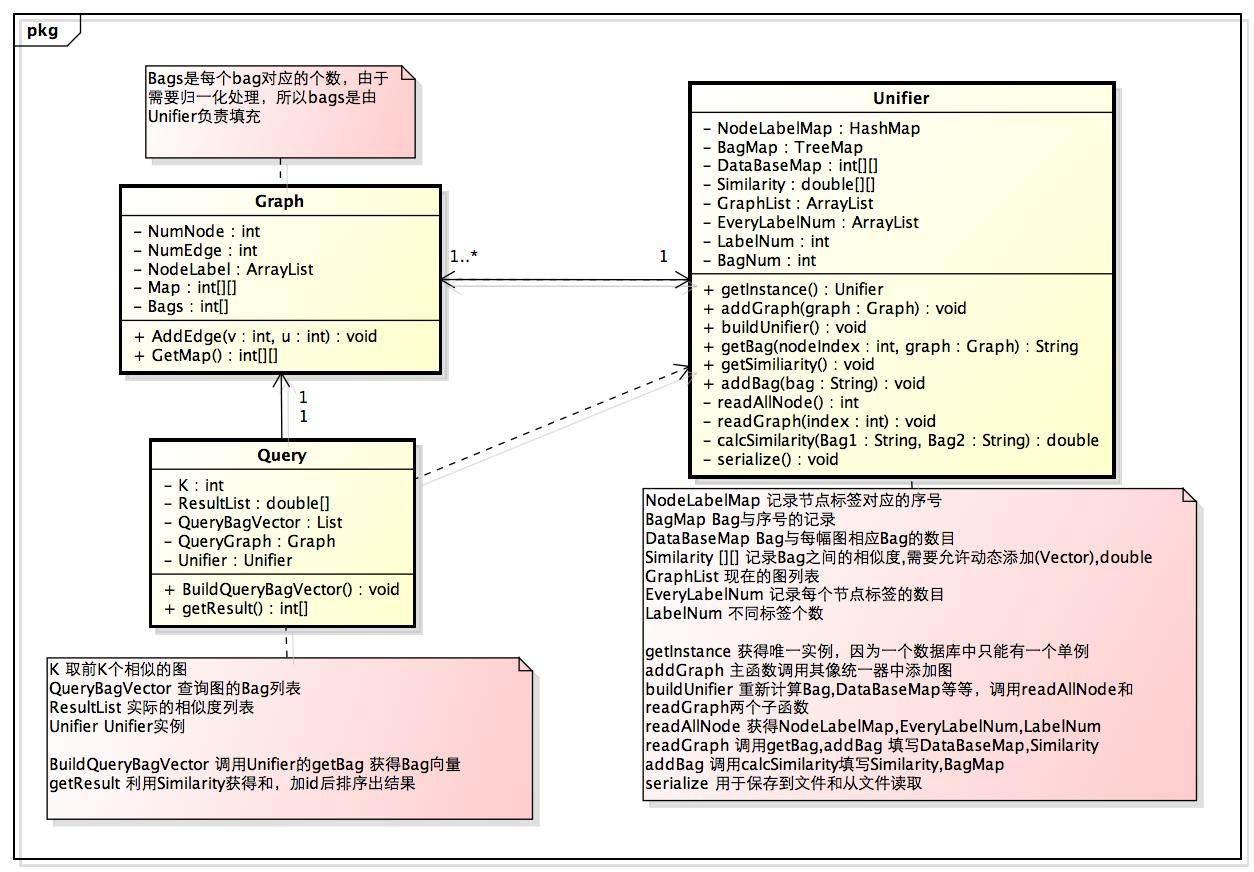
\includegraphics[width=\textwidth ]{../figures/G-Hash-pkg}
    \caption{基于节点相似度的图相似性搜索设计类图}
    \label{fg:ghashdesign}
\end{figure}

其中,$Graph$为一个最小单元即一个图,对外提供一些基本数据访问方法。$Unifier$顾名思义,是个用于归一化的类,也是数据库类,负责建库,增删图,和数据查询时一些算法定义,像获取简化包表示,图相似度计算就是靠这个类实现的。$Query$是一个查询,通过调用$Unifier$实现查询过程,最后输出查询结果。结果表现为图的id列表。我们还给$Unifier$添加了序列化接口,实现建库查询分离,加速查询过程。

由上可见,基于节点相似度的图相似算法实现非常方便,可运用在大量环境中。


\section{实验结果与分析}
\subsection{实验环境}
本文提出算法的实验环境为CPU Intel Core i7,主频为1.7 GHz,内存为8 GB 1600 MHz DDR3,硬盘为128GB SSD,操作系统为Mac OS X Yosemite 10.10.3;所有算法均用Java语言在JDK1.7u71环境编译完成。
\subsection{实验数据分析}
实验数据全采用真实数据,为DTP提供的AIDS数据集。可从以下网址得到:\url{https://wiki.nci.nih.gov/display/NCIDTPdata/AIDS+Antiviral+Screen+Data}。我们从其数据库中随机抽取了1000,2000,4000,8000,16000个图作为我们的查询集合。数据集平均每幅图有41条节点,48条边。所有实验运行10次取平均值。由于未能联系到原作者,实验中用于对照的G-Hash算法也是我们根据G-Hash论文\cite{ghash}自行仿写的。
\begin{figure}[htb]
    \centering
    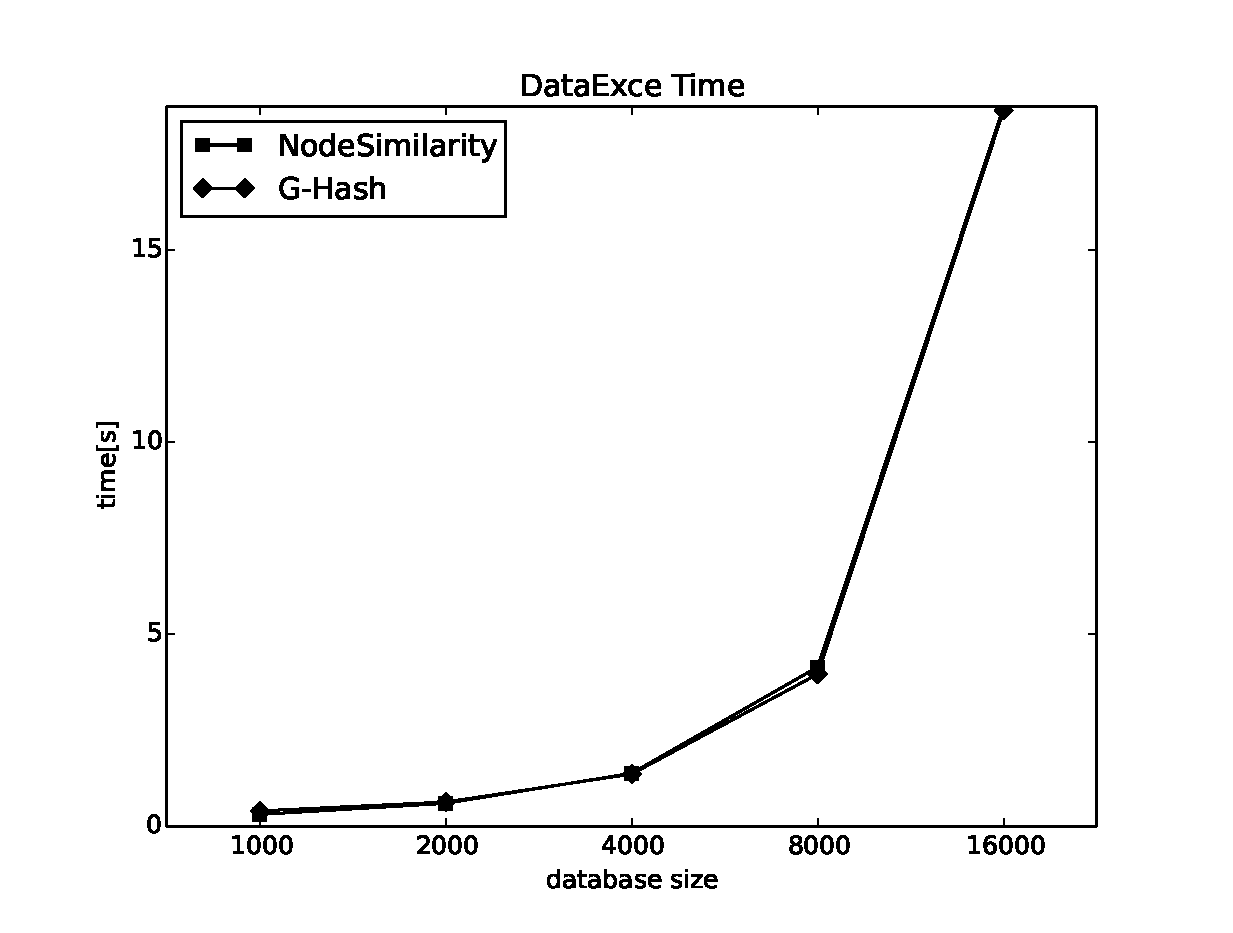
\includegraphics[width=0.6\textwidth]{../figures/THC/G-Hashcomapre}
    \caption{查询时间对比图}
    \label{fg:ghashtime}
\end{figure}

实验结果如图\ref{fg:ghashtime}所示,可以看出节点相似度算法与G-Hash算法在线查询时间基本一致,说明其性能不输于G-Hash算法,但是编码难度大大降低。由于近似搜索的精度并不好定义,因此我们没有给出精度的对比图。不过由于G-Hash靠哈希函数获得相似节点,具有局限性。而本算法则是完全计算所有节点相似度,显然更加可靠。

\ifx\allfiles\undefined
%\bibliographystyle{unsrt}
\bibliography{main}
\end{document}
\fi